\usetikzlibrary{positioning}
 \usetikzlibrary{decorations.pathreplacing,intersections}
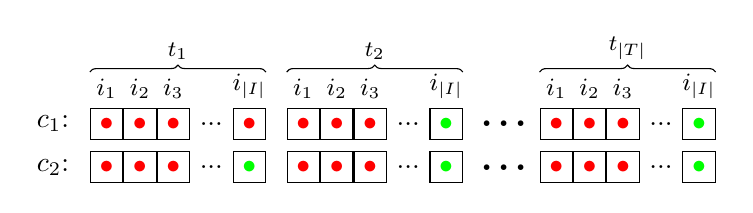
\begin{tikzpicture}

\node[rectangle,draw, label={\small $i_1$}] (c1i1) at (0,0) {\textcolor{red}{$\bullet$} };

\node[left=4pt of c1i1]  (c1) {\textcolor{black}{$c_1$:} };
  
\node[right=0pt of c1i1, rectangle,draw, label={\small $i_2$}] (c1i2) {\textcolor{red}{$\bullet$} };

\node[right=0pt of c1i2, rectangle,draw, label={\small $i_3$}] (c1i3) {\textcolor{red}{$\bullet$} };

\node[right=0pt of c1i3, ] (c1i4) {...};

\node[right=0pt of c1i4, rectangle,draw, label={\small $i_{|I|}$}] (c1i5) {\textcolor{red}{$\bullet$} };

\draw[decorate, decoration ={brace,raise=13pt}] (c1i1.north west) -- (c1i5.north east)
            node (subclauselabel) [midway, above=14pt] {\footnotesize{$t_1$}};


\node[rectangle,draw, label={\small $i_1$}] (c1i1) at (2.5,0) {\textcolor{red}{$\bullet$} };
  
\node[right=0pt of c1i1, rectangle,draw, label={\small $i_2$}] (c1i2) {\textcolor{red}{$\bullet$} };

\node[right=0pt of c1i2, rectangle,draw, label={\small $i_3$}] (c1i3) {\textcolor{red}{$\bullet$} };

\node[right=0pt of c1i3, ] (c1i4) {...};

\node[right=0pt of c1i4, rectangle,draw, label={\small $i_{|I|}$}] (c1i5) {\textcolor{green}{$\bullet$} };

\draw[decorate, decoration ={brace,raise=13pt}] (c1i1.north west) -- (c1i5.north east)
            node (subclauselabel) [midway, above=14pt] {\footnotesize{$t_2$}};

\node[right=2pt of c1i5, ] (v1) {\Huge{...}};

\node[right=0pt of v1, rectangle,draw, label={\small $i_1$}] (c1i1tN) {\textcolor{red}{$\bullet$} };

\node[right=0pt of c1i1tN, rectangle,draw, label={\small $i_2$}] (c1i2tN) {\textcolor{red}{$\bullet$} };

\node[right=0pt of c1i2tN, rectangle,draw, label={\small $i_3$}] (c1i3tN) {\textcolor{red}{$\bullet$} };

\node[right=0pt of c1i3tN, ] (c1i4tN) {...};

\node[right=0pt of c1i4tN, rectangle,draw, label={\small $i_{|I|}$}] (c1i5tN) {\textcolor{green}{$\bullet$} };

\draw[decorate, decoration ={brace,raise=13pt}] (c1i1tN.north west) -- (c1i5tN.north east)
            node (subclauselabel) [midway, above=14pt] {\footnotesize{$t_{|T|}$}};


  



% Contract 2



\node[rectangle,draw] (c2i1t1) at (0,-0.55) {\textcolor{red}{$\bullet$} };
  
\node[left=4pt of c2i1t1]  (c2) {\textcolor{black}{$c_2$:} };
  
\node[right=0pt of c2i1t1, rectangle,draw] (c2i2t1) {\textcolor{red}{$\bullet$} };

\node[right=0pt of c2i2t1, rectangle,draw] (c2i3t1) {\textcolor{red}{$\bullet$} };

\node[right=0pt of c2i3t1 ] (c2i4t1) {...};

\node[right=0pt of c2i4t1, rectangle,draw] (c2i5t1) {\textcolor{green}{$\bullet$} };



\node[rectangle,draw] (c2i1t2) at (2.5,-0.55) {\textcolor{red}{$\bullet$} };
  
\node[right=0pt of c2i1t2, rectangle,draw] (c2i2t2) {\textcolor{red}{$\bullet$} };

\node[right=0pt of c2i2t2, rectangle,draw] (c2i3t2) {\textcolor{red}{$\bullet$} };

\node[right=0pt of c2i3t2, ] (v2) {...};

\node[right=0pt of v2, rectangle,draw] (c2iNt2) {\textcolor{green}{$\bullet$} };



\node[right=2pt of c2iNt2, ] (v3) {\Huge{...}};


\node[right=0pt of v3, rectangle,draw] (c2i1tN) {\textcolor{red}{$\bullet$} };

\node[right=0pt of c2i1tN, rectangle,draw] (c2i2tN) {\textcolor{red}{$\bullet$} };

\node[right=0pt of c2i2tN, rectangle,draw] (c2i3tN) {\textcolor{red}{$\bullet$} };

\node[right=0pt of c2i3tN, ] (c2i4tN) {...};

\node[right=0pt of c2i4tN, rectangle,draw] (c2i5tN) {\textcolor{green}{$\bullet$} };


\end{tikzpicture}